\chapter{Comportamiento dinámico y estabilidad}
El concepto de estabilidad y su análisis constituye unos de los aspectos claves para el estudio de los sistemas dinámicos. La estabilidad de un sistema esta estrechamente relacionada con su comportamiento dinámico y puede definirse de diversas maneras. En este capítulo nos centraremos en el análisis de los llamados puntos de equilibrio de un sistema y los estudiaremos de acuerdo con el concepto de estabilidad de Lyapunov. Además, incidiremos en otros aspectos de la estabilidad de los sistemas tales como la existencia de ciclos límite o el movimiento nominal. Empecemos pues por enunciar algunas definiciones de estabilidad.



\section{Estabilidad de un sistema dinámico}
Dado un sistema dinámico no forzado,
\begin{align}
\dot{x} = f(t,x) \label{eq: sis1}\\
y = g(t,x)
\end{align}

\begin{definition}[Estabilidad de las soluciones de un sistema dinámico]
Una solución $x(t;x_0)$ para la condición inicial $x(0) = x_0$ se dice que es estable si  $\exists R>0$ y  $ \exists r>0$ tal que, dada otra condición inicial $\hat x_0$ se verifica,
\begin{equation}
\|\hat x_0-x_0\|<r \Rightarrow \|x(t;\hat x_0) - x(t;x_0)\|<R, \forall t \geq 0
\end{equation}

En otro caso se dice que la solución es inestable 
\qed
\end{definition}

\begin{definition}[Estabilidad asintótica]
Una solución $x(t;x_0)$ para el sistema \ref{eq: sis1} se dice que es asintoticamente estable si es estable y además  $\exists r>0$, tal que dada otra condición inicial $\hat x_0$ se verifica,
\begin{equation}
\|\hat x_0-x_0\|<r \Rightarrow \lim_{t \to \infty}\|x(t;\hat x_0) - x(t;x_0)\|=0
\end{equation}

es decir, cualquier solución con condición inicial próxima  a $x(t;x_0)$ converge a $x(t;x_0)$
\qed
\end{definition}

\begin{definition}[Estabilidad marginal]
Una solución que es estable, pero no asintóticamente estable, se denomina marginalmente estable
\qed
\end{definition}

\begin{definition}[Estabilidad exponencial]
Una solución $x(t;x_0)$ para el sistema \ref{eq: sis1} se dice que es exponencialmente estable estable si es estable y además  $\exists r>0$, tal que dada otra condición inicial $\hat x_0$ se verifica que existen $\alpha>0 , \sigma >0$, tales que,
\begin{equation}
\|\hat x_0-x_0\|<r \Rightarrow \|x(t;\hat x_0) - x(t;x_0)\| \leq \|\hat x_0 - x_0\| \alpha e^{-\sigma t}
\end{equation}
\qed
\end{definition}

Por último indicar que cuando la estabilidad se cumple para cualquier condición inicial, $\hat x  \in \mathbb{R}^n$ la solución $x(t;x_0)$ se denomina \emph{globalmente} estable.


\subsection{Puntos de equilibrio} 
\begin{definition}[Punto de equilibrio] Dados un sistema dinámico definido por las ecuaciones,
\begin{align}
\dot{x} = f(x,u)\\
y = g(x,u)
\end{align}
donde $x \in \mathbb{R}^n$, $u \in \mathbb{R}^m$ e $y \in \mathbb{R}^l$. Se definen como puntos de equilibrio o puntos estacionarios los valores del vector de estados $\overline x$ y del vector de entradas $\overline u$ para los cuales el estado y, consecuentemente, la salida del sistema permanecen constantes,

\begin{align}
\dot{\overline x} \equiv 0 = f(\overline x, \overline u)\\
\overline y = g(\overline x,\overline u)
\end{align}
\qed
\end{definition}

Si el vector de estados no cambia, su derivada será cero. Por tanto, mientras no se altere el valor de la entrada, el sistema permanecerá en el mismo estado y el valor del vector de salidas permanecerá también constante. 

Podemos, a partir de esta definición, obtener algunas propiedades importantes de los puntos de equilibrio:
\begin{enumerate}
\item Una vez que un sistema alcanza un punto de equilibrio, permanece en él indefinidamente. (Todas las derivadas temporales de las componentes del vector de estado son cero.
\item Desde el punto de vista del control de sistemas, los puntos de equilibrio juegan un papel importante ya que representan condiciones de operación constante.
\item Un sistema dinámico puede tener uno o más puntos de equilibrio, o no tener ninguno. 
\end{enumerate}

\paragraph{Sistemas autónomos.} Para simplificar el estudio de la estabilidad, podemos empezar por considerar el casos de sistemas autónomos con entrada nula  $u = 0, \ \forall t$. La salida evoluciona a partir de un estado inicial $x_0\equiv x(t_0)$,

\begin{align}
\dot{x} = f(x)\\
y = g(x)
\end{align}

\paragraph{Sistemas realimentados.} Del mismo modo, podemos considerar sistemas en los que la entrada es una función directa del valor de los estados; $\textbf{u}= \textbf{c(x)}$. Hablaremos entonces de un \emph{sistema realimentado}. A efectos de análisis de la estabilidad del sistema, no hay diferencia entre un sistema realimentado y un sistema autónomo,
\begin{align}
\dot{x} = f(x,c(x)) = \bar{f}(x)\\
y = g(x,c(x)) = \bar{g}(x)
\end{align}
El nombre de sistema realimentado, proviene de considerar que se están \emph{realimentando} los estados en la entrada del sistema. El concepto de realimentación constituye uno de los pilares de los sistemas de control. La figura \ref{fig:rea}, muestra esquemáticamente este concepto.

\begin{figure}
\centering
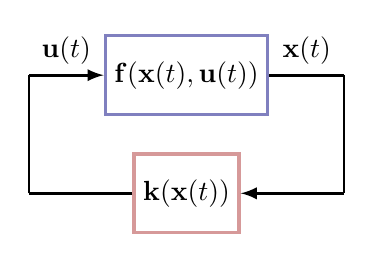
\begin{tikzpicture}
\draw(0,0) node(p)[rectangle, minimum height=10mm, minimum width=10mm,align=center, very thick, draw = blue!50!black!50]{$\mathbf{f}(\mathbf{x}(t),\mathbf{u}(t))$}

(0,-1.5) node(c)[rectangle, minimum height=10mm, minimum width=10mm,align=center ,very thick,draw = red!60!black!40]{$\mathbf{k}(\mathbf{x}(t))$};

\draw[line width = 1pt](p)--(2,0)node[midway,above]{$\mathbf{x}(t)$};
\draw[line width = 1pt](2,0)--(2,-1.5);
\draw[line width = 1pt, -latex](2,-1.5)--(c);
\draw[line width = 1pt](c)--(-2,-1.5);
\draw[line width = 1pt](-2,-1.5)--(-2,0);
\draw[line width = 1pt, -latex](-2,0)--(p)node[midway,above]{$\mathbf{u}(t)$};

\end{tikzpicture}

\caption{Esquema general de un sistema realimentado}\label{fig:rea}
\end{figure}

\section{Estabilidad de Lyapunov}
 En esta sección vamos a centrarnos en el estudio de la estabilidad de los puntos de equilibrio. 

Habitualmente, cuando se trata de la estabilidad de los puntos de equilibrio se suele hablar de estabilidad en el \emph{sentido} de Lyapunov. Aleksandr Mikhailovich Lyapunov un matématico ruso, de finales del siglo XIX, que estableció los fundamentos de la teoría de la estabilidad que ahora lleva su nombre.

Un punto de equilibrio de un sistema dinámico es \emph{estable} si toda  solución que comienzan cerca del punto de equilibrio permanece cercana al punto de equilibrio; en otro caso, el punto de equilibrio es inestable. Es \emph{asintóticamente estable} si toda solución que empieza próxima al punto de equilibrio no solo permanecen cerca del punto de equilibrio sino que tienden a él cuando el tiempo tiende a infinito.

Podemos relacionar directamente la estabilidad de un punto de equilibrio, con la estabilidad de las trayectorias de un sistema lineal definida en () i consideramos  un punto de equilibrio como una solución del sistema dinámico, cuya condición inicial es el propio punto de equilibrio: $x(t;\overline x) = \overline x$.

\subsection{Estabilidad de Lyapunov para sistemas autónomos}
Consideremos un sistema autónomo genérico,
\begin{equation}\label{eq: aut}
\dot x = f(x),
\end{equation}
donde $f(x): D\rightarrow \mathbb{R}^n$ es una función (localmente) lipschitziana desde un domino $D \subset \mathbb{R}^n$ a $\mathbb{R}^n$. Supongamos además que $\overline x \in D$ es un punto de equilibrio; es decir, $f(\overline x) = 0$. Lo que buscamos es un método para caracterizar el tipo de estabilidad de $\overline x$. En lo que sigue, y sin perdida de generalidad, consideramos que el punto de equilibrio es es origen de coordenadas $\overline x = 0$ \footnote{Siempre es posible hacer un cambio de coordenadas de modo que si $\overline x \neq 0$, $z = x-\overline x$; $\dot z = \dot x = f(x+\overline x) := g(z)$, donde $g(0)=0$.}.

\begin{definition} (Estabilidad de Lyapunov, para un punto de equilibrio)\label{def: est}
El punto de equilibrio x = 0 del sistema \ref{eq: aut} es:
\begin{itemize}
\item estable $\forall \epsilon > 0$ que cumpla:
\begin{equation*}
 \exists \delta =\delta(\epsilon)>0: \| x(0) \| < \delta \Rightarrow \| x(t)\| < \epsilon \ \forall t \ge 0
\end{equation*}
 
 \item Es inestable si no es estable.
 \item Es asintóticamente estable si es estable y además se puede elegir $delta$ de modo que,
\begin{equation*}
\| x(0)\| < \delta \Leftarrow \lim_{t \to \infty} x(t) = 0
\end{equation*}
\end{itemize}
\qed
\end{definition}

En 1892 Lyapunov propuso un método para analizar la estabilidad de un punto de equilibrio, basado en el análisis  una función $V:D\to \mathbb{R}$, continua y diferenciable en un entorno $D \subset \mathbb{R}^n$. En concreto, el método analiza la variación de la función $V$ a lo largo de las \emph{trayectorias} del sistema cuya estabilidad se quiere analizar, Podemos representar dicha variación empleando la derivada temporal de la función $V$
\begin{equation} \label{eq: dlyap}
\dot V(x) = \sum_{i=0}^{n}\frac{\partial V}{\partial x_i} \dot x_i = \sum_{i=0}^{n}\frac{\partial V}{\partial x_i} f(x) = \nabla V(x)\cdot f(x)
\end{equation}

Es interesante hacer notar que, lógicamente, $\dot V$ depende del sistema que se desea analizar y que Si $\phi(t;x)$ es una solución del sistema \ref{eq: aut} , que empieza, como condición inicial, en estado $x$, para $t=0$ Entonces,
\begin{equation}
\dot V(x) =\left. \frac{d}{dt}V(\phi (t;x))\right|_{t=0},
\end{equation}
Por tanto, si $\dot V(x)$ es negativa, $V$ decrecerá a lo largo de la solución del sistema \ref{eq: aut}.

\begin{theorem}\label{thm: lyap1}
Sea $x=0$ un punto de equilibrio para el sistema \ref{eq: aut} y $D \subset \mathbb{R}^n$ un dominio que contiene a $x=0$. Sea $V:D 	\to \mathbb{R}$ una función continua y diferenciable tal que,
\begin{equation}\label{eq: lyap1}
V(0) = 0\ y\ V(x) > 0\ en\  D-\{0\},
\end{equation}
\begin{equation}\label{eq: lyap2}
\dot V(x) \leq 0\ en\ D,
\end{equation} 
entonces $x=0$ es estable de forma local. Además, si
\begin{equation}\label{eq: lyap3}
\dot V(x) < 0 \ en\ D-\{0\},
\end{equation} 
Entonces $x(0)$ es asintóticamente estable de forma local.
\end{theorem}
\begin{proof}
Dado $\epsilon > 0$, elegimos $r \ in (0,\epsilon]$ tal que,
\begin{equation*}
B_r = \left\{ x \in \mathbb{R} \ |\  \|x\| \leq r \right\} \subset D.
\end{equation*}
Sea $\alpha =  \min_{\|x\| = r}V(x)$. Donde, $\alpha >0$ de acuerdo con \ref{eq: lyap1}. Tomamos ahora $\beta \in (0,\alpha)$ y construimos un nuevo dominio de modo que,
\begin{equation*}
\Omega_\beta = \left\{ x \in B_r \ |\  V(x) \leq \beta \right\}
\end{equation*}
Pero entonces $\Omega_\beta$ está en el interior de $B_r$.  Si no fuera así, sería posible encontrar un $p \in \Omega_\alpha$ que estaría situado en la frontera $B_r$. Pero en este punto $V(p) \ge \alpha > \beta$, lo que estaría en contradicción con la definición de $\Omega_\beta$. 

El conjunto $\Omega_\beta$ tiene la propiedad, de que cualquier trayectoria del sistema que empiece en $\Omega_\beta$  en $t=0$ permanecerá en $\Omega_\beta, \forall t \geq 0$; ya que, de acuerdo con \ref{eq: lyap2}
\begin{equation*}
\dot V \leq 0 \Rightarrow V(x(t)) \leq V(x(t)) \leq \beta, \forall t \geq 0.
\end{equation*}

Como $V(x)$ es continua y $V(0) = 0$,

\begin{equation*}
\exists \delta > 0\  |\  \|x\| \leq \delta \Rightarrow V(x) < \beta
\end {equation*}

lo que implica que,
\begin{equation*}
B_\delta \subset \Omega_\beta \subset B_r
\end{equation*}
y
\begin{equation*}
x \in B_\delta \Rightarrow x(0) \in \Omega_\beta \Rightarrow x(t) \in B_r,
\end{equation*}
por tanto,
\begin{equation*}
\|x(0)\| < \delta \Rightarrow \|x(t)\|<r \leq \epsilon, \ t \geq 0
\end{equation*}

Lo cual demuestra que el punto $x=0$ es estable (ver definición: \ref{def: est}). 

Si además suponemos que se cumple \ref{eq: lyap3}, para demostrar que el sistema es asintóticamente estable, debemos probar que $x \to 0$ cuando $t \to \infty$; Condición que podemos reformular como, $\forall a >0, \exists T>0\ | \ \|x\| < a \ \forall t>T$. Pero, si repetimos nuestro razonamiento anterior, dato un valor $a>0$ siempre podremos encontrar un $b>0$ para el que se cumpla que $ \Omega_b \subset B_a$. Por tanto, es suficiente probar que $V$ alcanza el valor $0$ si nos movemos a lo largo de las trayectorias del sistema, $\lim_{t \to 0}V(x(t))=0$. Sabemos que $V(x(t))$ es monótona decreciente a lo largo de las trayectorias, y que está acotada inferiormente por cero.
\begin{equation}
\lim_{t \to 0}V(x(t)=c \geq 0
\end{equation}
Debemos demostrar que,  si se cumple \ref{eq: lyap3}, $c=0$. Vamos  demostrarlo por contradicción. Supongamos que $c>0$. Por continuidad de la función $V(x)$, $\exists d>0\ | \ B_d \subset \Omega_c$ pero entonces el límite $V(x(t))\to c>0$ implica que las trayectorias $x(t)$ se quedan fuera de la bola $B_d, \forall t \geq 0$. Si fijamos  un entorno $d \leq \|x\| \leq r$ exterior a $B_b$, $\dot V(x)$ deberá alcanzar un valor máximo, $-\gamma =\max_{d \leq \| x \| \leq r} \dot{V}(x)$. Además, por \ref{eq: lyap3} $-\gamma < 0$. Si integramos $\dot V$,
\begin{equation*}
V(x(t)) = V(x(0)) + \int_0^t \dot V(x(\tau))d\tau \leq V(x(0)) -\gamma t
\end{equation*}
Pero la expresión a la derecha del menor o igual, terminará por hacerse negativa, por lo que $c$ no puede ser mayor que 0.
\end{proof}
Algunas observaciones:
\begin{itemize}
\item Una función continua y diferenciable $V(x)$ que cumple las condiciones \ref{eq: lyap1} y \ref{eq: lyap2} recibe el nombre de función de Lyapunov.
\item La derivada $\dot V$, definida en la ecuación (\ref{eq: dlyap}) recibe el nombre de derivada de Lyapunov o derivada de Lie.
\item Una función $V(x)$ que satisface $V(0)=0$ y $V(x)>0$ para $x\neq 0$ en $D$, (\ref{eq: lyap1}), se dice que es definida positiva en $D$.Si la solo satisface $V(x)\geq 0$ para $x\neq 0$ en $D$, se dice que es semidefinida positiva en $D$.
\item Una función que cumple que $-V(x)$ es definida positiva/semidefinida positiva en $D$, se dice que es definida negativa/semidefinida negativa en $D$. Podríamos por tanto reescribir el teorema \ref{thm: lyap1} diciendo que el origen es un punto de equilibrio estable, para un sistema dinámico si existe una función diferenciable definida positiva $V(x)$ tal que $\dot V(x)$ es semidefinida negativa, y es asintóticamente estable si $\dot V(x)$ es definida negativa.
\item El teorema de Lyapunov puede aplicarse a un sistema siempre que encontremos una función $V(x)$ que satisfaga las condiciones del teorema con independencia de que conozcamos o no la solución del sistema.
\item El teorema \ref{thm: lyap1} aporta condiciones suficientes para la estabilidad de un sistema; el hecho de no ser capaz de encontrar una función de Lyapunov para un sistema dado, no implica necesariamente que este sea inestable. Solo muestra que no se puede establecer la estabilidad del sistema mediante la función e
\item Además, no es constructivo; indica que si existe una función de Lyapunov para el sistema, éste es estable, pero no indica cómo construir dicha función. 
\end{itemize}

El hecho de que no exista un método sistemático de determinar una función de Lyapunov para un sistema, hace que sea preciso en muchos casos probar con funciones 'candidatas' y comprobar sin cumplen las condiciones del teorema. Como idea general, en sistemas mecánicos y eléctricos una buena función candidata suele ser la energía del sistema. Una clase general de funciones para las que es fácil comprobar si son definidas positivas o no, lo constituyen las funciones cuadráticas,
\begin{equation}
V(x) = x^TPx = \sum_{i=1}^n \sum_{j=1}^n p_{ij}x_ix_j
\end{equation}
Donde $P$ es una matriz simétrica. $V(x)$ es entonces definida (semidefinida) positiva si todos los autovalores de $P$ son positivos (no negativos) o, lo que es equivalente, si todos los menores principales de $P$ son positivos.

\begin{example}[El péndulo invertido]
Volvamos de nuevo al ejemplo del péndulo invertido. Tomamos como punto de partida las ecuaciones (\ref{eq:pi1}), (\ref{eq:pi2}) propuestas en el capítulo anterior,
\begin{align*}
\dot x_1 = &x_2 \\ 
\dot x_2 = &\frac{g}{l}\sin x_1 - \frac{b}{ml}x_2 
\end{align*}
No tiene demasiado sentido estudiar la estabilidad del punto $(0,0)$, sabemos que no es estable y por tanto será imposible encontrar para él una función de Lyapunov válida. Podemos probar con el punto $(\pi,0)$ que sabemos que sí es estable. Para poder aplicar el método de Lyapunov necesitamos desplazar el punto de equilibrio al origen; $z_1=x_1-\pi,z_2=x_2$. Con lo que las ecuaciones del sistema quedan,
\begin{align*}
\dot z_1 = &z_2 \\ 
\dot z_2 = &-\frac{g}{l}\sin z_1 - \frac{b}{ml}z_2 
\end{align*}
Podemos emplear como función tentativa de Lyapunov la ``energía" del sistema,
\begin{equation*}
V(x) = \frac{1}{2}z_2^2 + \frac{g}{l}\left(1-\cos(z_1)\right)
\end{equation*}
Donde el término correspondiente a la ``energía potencial" se ha obtenido integrando el par de fuerza debido a la gravedad,
\begin{equation*}
-\int_0^{z_1}-\frac{g}{l}\sin(\zeta_1)d\zeta_1 =  \frac{g}{l}\left(1-\cos(z_1)\right)
\end{equation*}

Calculamos ahora la derivada de Lee para el péndulo invertido y la función elegida $V$,
\begin{equation*}
\dot V = \nabla V(x) \cdot f(x) = \begin{bmatrix}
\frac{g}{l}\sin(z_1) & z_2
\end{bmatrix} \cdot
\begin{bmatrix}
z_2\\
 -\frac{g}{l} \sin(z_1) - \frac{b}{ml}z_2 
\end{bmatrix}  = -\frac{b}{lm}z_2^2
\end{equation*}

Es fácil comprobar que $\dot V(z)$ es una función semidefinida negativa, $\dot V(z)=0$ a lo largo de todo el eje $z_2=0$, con independencia del valor que tome $x_1$, por tanto solo podemos afirmar que el punto de equilibrio $z=(0,0) \rightarrow x=(\pi,0)$ es estable. Sin embargo, si miramos el diagrama de fase de la figura \ref{fig:piphp} observamos que el sistema es asintóticamente estable. La función de Lyapunov elegida, no nos permite comprobarlo.

Podemos probar a modificar nuestra función de Lyapunov, sustituyendo la expresión de la energía cinética, por una forma cuadrática sobre ambas variables de estado:
\begin{equation*}
V(z) = \frac{1}{2} z^TPz+ \frac{g}{l}\left(1-\cos(z_1)\right)
\end{equation*}
Donde,
\begin{equation*}
P = \begin{bmatrix}
p_{11} & p_{12}\\ p_{12} & p_{22}
\end{bmatrix},
\end{equation*}
es una matriz simétrica definida positiva.
Si calculamos ahora la derivada de Lee,
\begin{equation*}
\dot V =\left(p_{12}-\frac{b}{lm}p_{22}\right)z_2^2+ \left(p_{11}-\frac{b}{lm}p_{12} \right) z_1z_2 + (1 -P_{22})\frac{g}{l} z_2\sin(z_1) + p_{12}\frac{g}{l} z_1\sin(z_1)
\end{equation*}
Podemos aprovechar la libertad que nos da poder elegir los elementos de $P$ para eliminar los téminos cruzados de la derivada de Lee, que contribuyen a que quede indefinido el signo. Si hacemos $p_{11} = \frac{b}{lm}p_{12}$ y $p_{22}=1$,
\begin{equation*}
\dot V =\left(p_{12}-\frac{b}{lm}\right)z_2^2-p_{12}\frac{g}{l} z_1\sin(z_1)
\end{equation*}
Necesitamos imponer condiciones adicionales  para asegurar que la matriz $P$ es definida positiva. Necesitamos que $p_{11}>0$ y que $\det(P)>0$, si sustituimos por los valores que ya hemos elegido,

\begin{equation*}
P =\begin{bmatrix}
\frac{b}{lm}p_{12} & p_{12}\\
p_{12} & 1
\end{bmatrix}, \ \det(p) = p_{12}\frac{b-lmp_{12}}{lm}
\end{equation*}

Debemos, por tanto, tomar $p_{12}$ en el intervalo,$0<p_{12}< \frac{b}{lm}$. Si elegimos por ejemplo $p_{12} =  \frac{b}{2lm}$, obtenemos para la derivada de Lee,
\begin{equation*}
\dot V =-\frac{b}{2lm}z_2^2-\frac{bg}{2l^2m}z_1 \sin(z_1)
\end{equation*}

Si tomamos un intervalo $D=\left\{x \in \mathbb{R}^2 \ | \ |x_1|<\pi \right\}$, la derivada de Lee es siempre negativa y, por tanto, podemos concluir que el origen es asintóticamente estable. Es interesante remarcar en este punto, que el teorema nos asegura no la estabilidad asintótica del origen, pero no nos dice nada de su dominio de atracción.

\qed
\end{example}


\subsection{Estabilidad asintótica global.}
El teorema \ref{thm: lyap1}, establece la estabilidad asintótica del origen de coordenadas, para un sistemas, en un entorno local incluido en $D$, si $\dot V(x) < 0.$.  Una pregunta inmediata que podemos plantearnos es, a qué distancia puede estar del origen una trayectoria sin dejar de ser asintóticamente estable. Es decir, que la trayectoria se aproxime al origen cuando $t$ tiende a $\infty$. Esto nos lleva a la definición de la región de atracción de un punto fijo, en particular, del origen.
\begin{definition}[Dominio de atracción.]
Sea $\phi(t;x)$ la solución de el sistema (\ref{eq: aut}) con condición inicial $x$ en el instante $t=0$ y supongamos además que el sistema tiene un punto de equilibrio asintóticamente estable, $\overline x$. Se define como región de estabilidad asintótica, dominio de atracción o cuenca de atracción de dicho punto al conjunto de todos los puntos $\{x\}$ tales que,
\begin{equation}
\lim_{t \to \infty} \phi(t;x) = \overline x
\end{equation}
\qed
\end{definition}

Determinar con exactitud la cuenca de atracción de un sistema puede resultar una tarea muy difícil o incluso imposible. Sin embargo el teorema de Lyapunov nos permite obtener una aproximación de la región de estabilidad asintótica; si tenemos una función de Lyapunov que cumple con las condiciones de estabilidad asintótica en un dominio $D$, y si $\Omega_c =\{x \in \mathbb{R}^n \vert V(x) \leq C$ Esta acotada e incluida en $D$,  Entonces toda trayectoria que empieza en $\Omega_c$ permanece en $Omega_c$ y, además se acerca al origen asintóticamente. Por tanto, podemos considerar $\Omega_c$ como una estima de la cuenca de atracción. Por supuesto, dicha estima puede resultar muy conservadora y, por  tanto, puede ser mucho menor que la cuenca de atracción.

Una segunda pregunta interesante sería determinar bajo qué condiciones un punto de equilibrio es \emph{asintóticamente estable de forma global}, es decir, cuando la cuenca de atracción de un punto de equilibrio asintóticamente estable es todo $\mathbb{R}^n$.  Para ello necesitamos imponer, en primer lugar que el dominio en que se cumplen las condiciones de la función $V(x)$ sea, $D=\mathbb{R}^n$. Además hay que imponer que   $V(x)$ sea una función no acotada radialmente:, $V(x) \to \infty$ cuando $\|x\| \to \infty$.

\begin{figure}
 \centering
 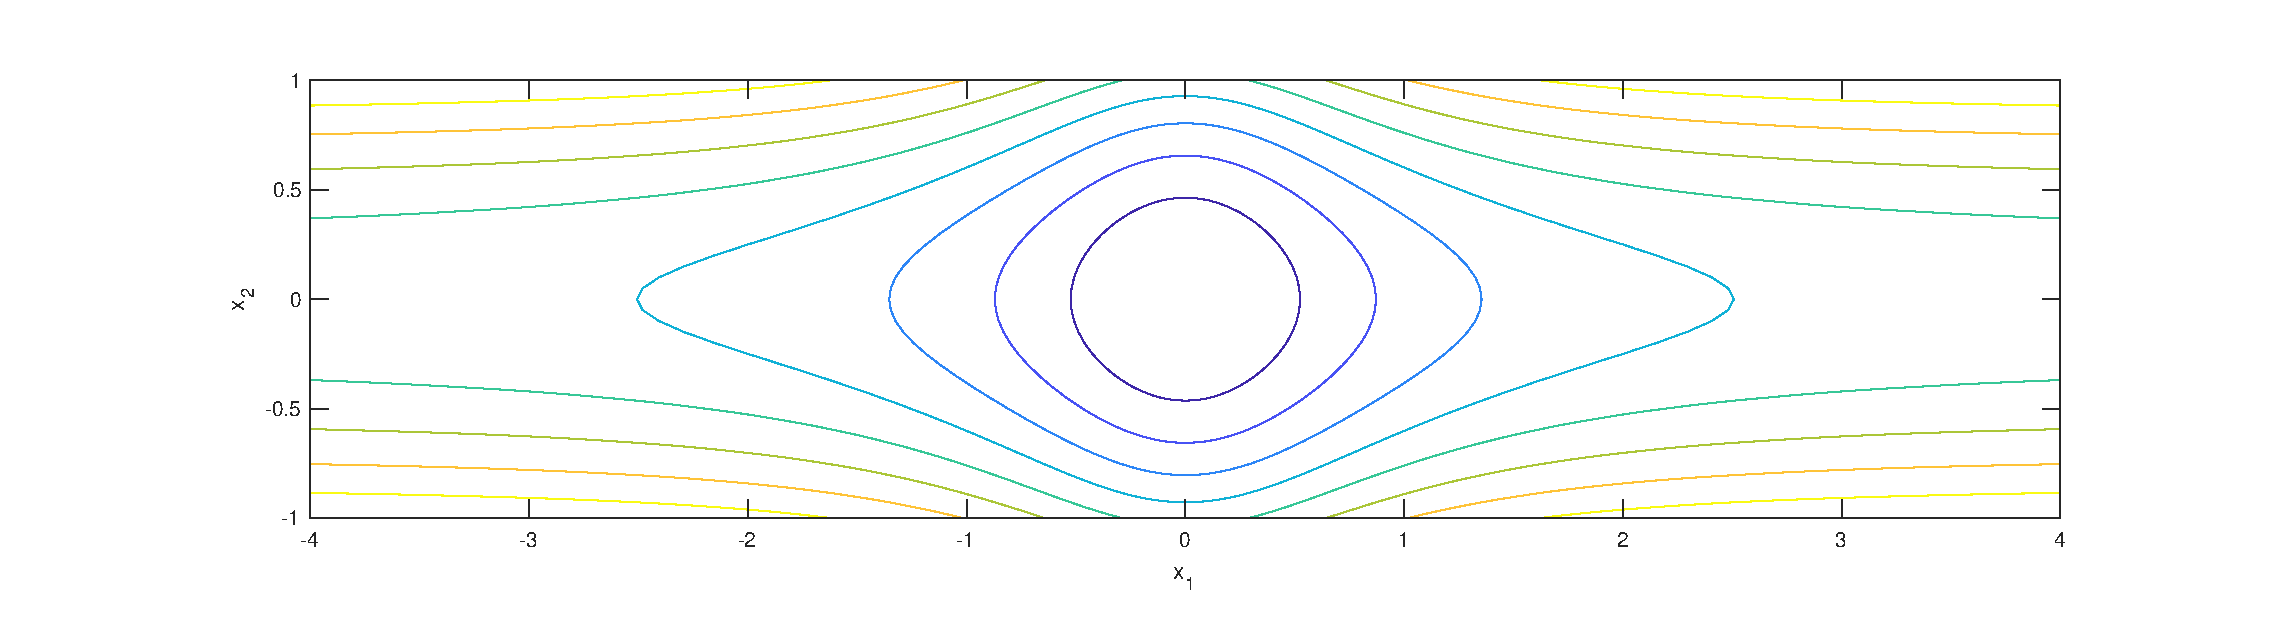
\includegraphics[scale=0.35]{radial_bounded.eps}
\caption{Curvas de nivel de $V(x) = \frac{x_1^2}{x_2^2+1}+x_2^2$}
\label{fig: radunb}
\end{figure}


\begin{theorem}\label{thm: BK}
Sea $x=0$ un punto de equilibrio para el sistema \ref{eq: lyap1}. Sea $V: \mathbb{R}^n \to \mathbb{R}$ una función continua y diferenciable tal que:
\begin{equation}
V(0) = 0\ y\ V(x) > 0\ \forall X,\  \neq 0 
\end{equation}
\begin{equation} \label{eq: BK2}
\|x\| \to \infty \Rightarrow V(x) \to \infty
\end{equation}
\begin{equation}
\dot V < 0, \forall x \neq 0
\end{equation}
Entonces $x=0$ es asintóticamente estable de forma global. 
\end{theorem} 
\begin{proof}
Dado un punto cualquiera $p \in \mathbb{R}^n$, sea $c = V(c)$. La condición \ref{eq: BK2} implica que $\forall c>0,\ \exists r>0,\ \vert V(x) > c$ siempre que $\|x\| >r$. Por tanto $\Omega_c \subset B_r$, y por tanto está acotado. El resto de la prueba es igual que la del teorema \ref{thm: lyap1}.
\end{proof}

El teorema \ref{thm: BK} se conoce con el nombre de teorema de Barbashin-Krasovskii. Es fácil observar que si un sistema posee un punto de equilibrio $\overline x_1 $ asintóticamente estable de forma global, dicho punto de equilibrio es único. Efectivamente si el sistema tuviera un segundo punto de equilibrio $\overline x_2$ cualquier trayectoria que empezara en $\overline x_2$ permanecería en dicho punto $\forall t\geq 0$, contradiciendo por tanto la definición de equilibrio global para $\overline x_1$.

Es importante remarcar la importancia de que $V(x)$ sea una función no acotada radialmente. La razón está en que para probar tanto el teorema de Lyapunov como el de Barbashin-Krasovskii necesitamos poder construir un entorno acotado, incluido en una bola $B_r$ en torno al origen, $\Omega_e$ en el que la función $V(x) \leq e$. El problema es que ahora necesitamos encontrar dicho entorno, cualquiera que sea $x$. Eso supone que $V(x)$ debe crecer en cualquier dirección que escojamos para alejarnos del origen $\|x\| \to \infty$. Veamos un ejemplo de una  función que no lo hace, 
\begin{equation*}
V(x) = \frac{x_1^2}{x_1^2+1}+x_2^2
\end{equation*}
 La función cumple que $V(0) = 0$ y $V(x) >0\ \forall x>0$. Sin embargo, es fácil ver que, si nos alejamos del origen a lo largo del eje$(x_1,0)$,
 \begin{equation}
 \lim_{x1\to\infty,x2=0} \frac{x_1^2}{x_1^2+1}+x_2^2 = 1
 \end{equation}
 Por tanto, como muestra la figura \ref{fig: radunb}, es imposible encontrar una curva de nivel cerrada, para la que $V(x) >1$, y por tanto no podemos emplear la función fuera de la bola $B_r(x)\ \vert\ , \|x\| \leq 1$.
 
\subsection{Interpretación geométrica del teorema de Lyapunov.}
\begin{figure}
\subfigure[Función $V(x) = X_1^2+X_2^2$.]{
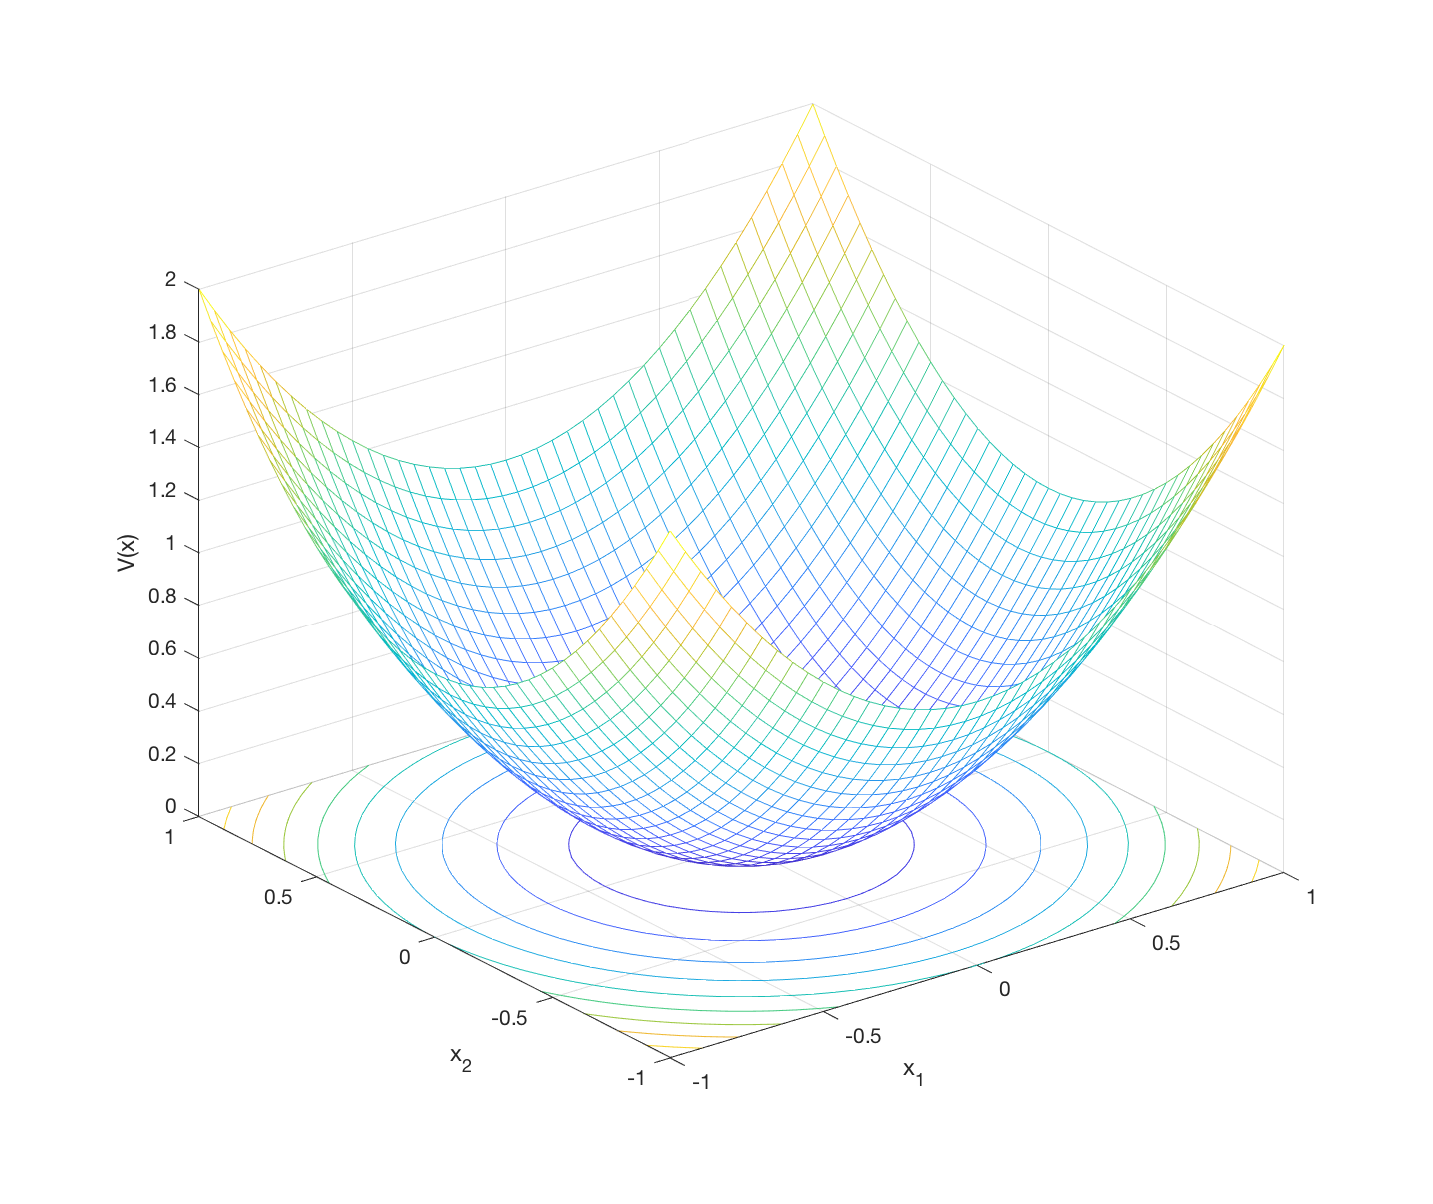
\includegraphics[scale=0.3]{lyapunov_v.eps}}
\subfigure[Curvas de nivel de $V(x) = X_1^2+X_2^2$, gradiente $\nabla V(x)$ (flechas azules) y valor de $\dot x = f(x)$ en un punto (flecha roja).]{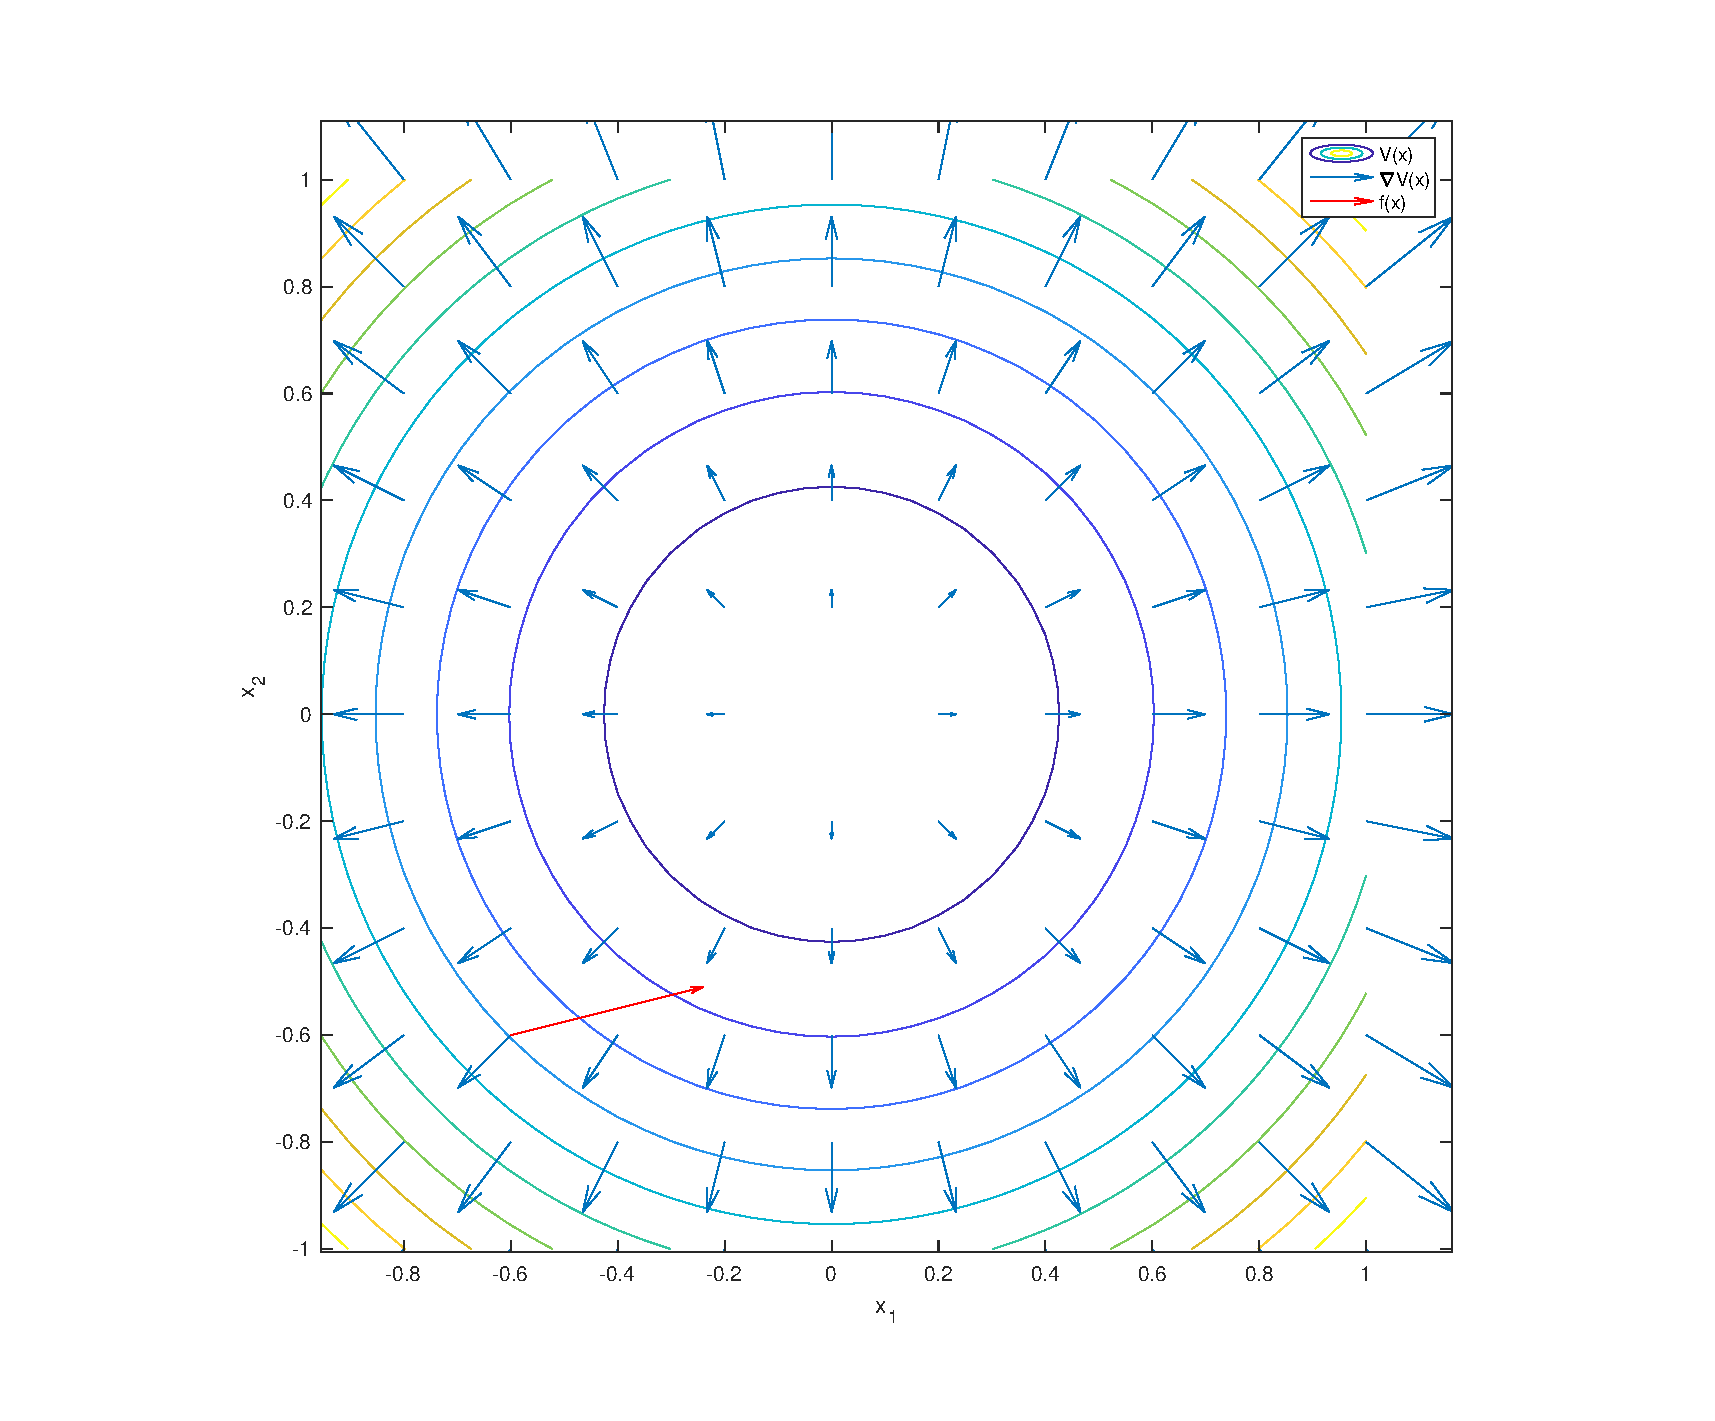
\includegraphics[scale=0.25]{lyapunov_nivel.eps}}
\caption{Interpretación geométrica de las condiciones de Lyapunov.}
\label{fig: lyap}
\end{figure}
 La figura \ref{fig: lyap} muestra un caso sencillo de las condiciones de Lyapunov. Supongamos que elegimos la función, definida positiva,  $V(x) = x_1^2 + x_2^2$ como candidata de Lyapunov para un sistema genérico $\dot x = f(x)$.  Para que el sistema sea estable, debe cumplirse que la derivada de Lie, ecuación  (\ref{eq: dlyap}), sea menor o igual que cero.  Pero esta derivada es en cada punto del espacio de fases el producto escalar del gradiente de $V$ por el valor de campo vectorial $f$ en dicho punto. Si dicho producto es negativo supone que el ángulo entre el gradiente y el valor del campo en dicho punto es mayor de $90º$, tal y como se muestra en la figura. Por tanto, la dirección del campo, lleva al sistema a acercarse al origen. Si el valor del producto es cero, indica que la dirección del campo es tangente a la curva de nivel de  $V(x)$ en el punto. Si en una región cerrada en torno al origen $\dot V \leq 0$ el sistema, una vez que entra en dicha región, no volverá a salir nunca más.
 Podríamos generalizar el resultado a sistemas de más dimensiones. Las curvas de nivel  $V(x)=c, c \in \mathbb{R} $, pasan a ser superficies de nivel, la condición de Lypianuv impone, por tanto, que una vez cruzada una superficie de nivel de $V(x)$ el sistema no sale de la región limitada por dicha superficie.
 
\section{Principio de invarianza de LaSalle}

\begin{definition}[Conjunto límite positivo]
Sea $x(t)$ una solución del sistema \ref{eq: sis1}. Un punto $p$ se dice que es un punto límite positivo de $x(t)$ si existe una secuencia $\{t_n\}$, con $t_n\to \infty$ cuando $n\to \infty$ tal que $x(t_n) \to p$ cuando $n \to \infty$.

Al conjunto de todos los puntos límite positivos se le denomina el conjunto límite positivo, $L^+$ de $x(t)$

\qed
\end{definition}

\begin{definition}[Conjunto invariante]
Un conjunto $M$ se dice que es invariante respecto al sistema \ref{eq: sis1}  si,
\begin{equation*}
x(0) 	\in M \Rightarrow x(t) \in M,\ \forall t \in \mathbb{R}.
\end{equation*}
Si cumple al menos,
\begin{equation*}
x(0) 	\in M \Rightarrow x(t) \in M,\ \forall t \geq 0,
\end{equation*}
entonces se dice que el conjunto $M$ es \emph{positivamente} invariante.
\qed
\end{definition}

Por tanto para un conjunto invariante $M$, si una solución pertenece a $M$ en un instante de tiempo, entonces también pertecenece a $M$ en todo instante pasado o futuro. Además para el caso de invarianza positiva, podemos decir que $x(t)$ se aproxima al conjunto $M$ cuando t tiende a infinito si para cada $\epsilon >0$,  hay un $T>0$ de modo que se cumple,
\begin{equation*}
\text{dist}(x(t),M)<\epsilon, \forall t>0,
\end{equation*} 
donde $\text{dist}(p,M)$ representa la distancia desde desde el punto $P$ al conjunto $M$, es decir, la distancia más corta desde $P$ a un punto cualquiera de $M$,
\begin{equation}
\text{dist}(p,M) = \inf_{x\in M}\|p-x\|
\end{equation} 

Esto conceptos nos permiten describir un punto de equilibrio asintóticamente estable como el conjunto límite positivo de cualquier solución suficientemente cercana a dicho punto. Un ciclo límite estable, sería el conjunto límite positivo de cualquier solución que comienza suficientemente cerca del ciclo límite. Además, el punto de equilibrio y el ciclo límite son conjuntos invariantes, ya que toda solución que empieza en ellos, permanece en ellos $\forall t \in \mathbb{R}$. El conjunto $\Omega_c =\{x \in \mathbb{R}^n\ |\ V(x)\leq c\}$ para el que se cumple $\dot V \leq c\ \forall x \in \Omega_c$ es un conjunto invariante positivo puesto que (ver teorema \ref{thm: lyap1}) puesto que cualquier solución que empieza en $\Omega_c$ permanece en $\Omega_c, \ \forall t \leq 0$.

\begin{lemma}[Sin demostración]\label{lem: L+}
Si una solución $x(t)$ de \ref{eq: aut}  está acotada, y pertenece a $D$ para $t \geq 0$ entonces su conjunto límite positivo  $L^+ \neq \emptyset$ es un conjunto invariante compacto. Además, $x(t)$ se aproxima a $L^+$ cuando $t \to \infty$.
\qed
\end{lemma}

\begin{theorem}\label{thm: LS}
Sea $\Omega \subset D$ un conjunto compacto positivamente invariante  con respecto al sistema \ref{eq: aut}. Sea $V:D\to \mathbb{R}$ una función continua y diferenciable tal que $\dot V \leq 0$ en $\Omega$. Sea $E$ el conjunto de todos los puntos de $\Omega$ para los cuales $\dot V = 0$. Sea $M$ el mayor conjunto invariante en $E$. Entonces, toda solución que empieza en $\Omega$ se aproxima a $M$ cuando $t\to \infty$
\end{theorem}
\begin{proof}
Sea $x(t)$ una solución de \ref{eq: aut} que comienza en $\Omega$,  Puesto que $\dot V\leq 0$ en $\Omega$, $V(x(t)$ es una función decreciente de $t$. Además, dado que $V(x)$ es una función continua en en el conjunto compacto $t$, la función está acotada inferiormente en $\Omega$. Por tanto,  $V(x(t))$ tienen un límite $a$ cuando $t\to \infty$. Por último el conjunto límite positivo de $x(t)$: $L^+ \subset \Omega$, puesto que $	\Omega$ es un conjunto cerrado.  Para cualquier $p \in L^+, \exists \{t_n\}$ con $n\to \infty \ | \ x(t_n)\to p$ cuando $n\to \infty$. Pero, por continuidad de $V(x)$, $V(p)= \lim{n\to \infty }V(x(t_n)=a$. Por tanto $V(x)=A$ en $L^+$. Puesto que (por el lema \ref{lem: L+}) $L^*$ es un conjunto invariante, $\dot V(x) = 0$ en $L^+$, Así que,
\begin{equation*}
L^+ \subset M \subset E \subset \Omega 
\end{equation*} 

Como $x(t)$ está acotada, x(t) se aproxima a a $L^+$ cuando $t\to \infty$ (lema \ref{lem: L+}), y por tanto, $x(t)$ se aproxima a $M$ cuando $t\to \infty$. 
\end{proof}

El teorema \ref{thm: LS} se conoce con el nombre de Teorema de LaSalle. Es interesante hacer notar que el teorema no exige, como en el caso del teorema de Lyapunov que la función $V(x)$ sea definida positiva. Si imponemos esta condición, podemos obtener dos modificaciones del teorema de LaSalle que nos permiten determinar la estabilidad asintótica de un sistema.

\begin{corollary}[Teorema de Barbashim-Krasovskii  I \protect\footnote{Hay tres teoremas debidos a los mismos autores, todos ellos relacionados con estabilidad asintótica. Los dos que se definen aquí, fueron demostrados por sus autores con anterioridad al teorema de LaSalle. Después de la demostración de éste último, quedaron como simples corolarios}]
Sea $x=0$ un punto de equilibrio asintóticamente estable para el sistema \ref{eq: aut}. Sea $V:D\to 	\mathbb{R}$ una función continua, diferenciable, definida positiva en el dominio $D$, que contiene al origen $x=0$, tal que $\dot V(x) \leq 0$ en $D$. Sea el conjunto $S=\{ x \in D\ |\ \dot V(x) = 0 \}$ y supongamos que no hay ninguna solución que pueda permanecer en $S$, excepto la solución trivial $x(t)=0$. Entonces el origen es asintóticamente estable.
\qed
\end{corollary}

\begin{corollary}[Teorema de Barbashim-Krasovskii II]
Sea $x=0$ un punto de equilibrio para el sistema \ref{eq: aut}. Sea $V:\mathbb{R}^n \to \mathbb{R}$ una función continua, diferenciable, no acotada radialmente y definida positiva, tal que $\dot V(x) \leq 0 \forall x \in \mathbb{R}^n$.  Sea el conjunto $S=\{ x \in D\ |\ \dot V(x) = 0 \}$ y supongamos que no hay ninguna solución que pueda permanecer en $S$, excepto la solución trivial $x(t)=0$. Entonces el origen es asintóticamente estable de modo global.
\qed
\end{corollary}

\section*{Ejercicios}
\begin{enumerate}
\item Encontrar los puntos singulares de los siguientes sistemas. Linealizar las ecuaciones en su entorno y determinar la naturaleza de dichos puntos singulares.
\begin{enumerate}
\item \begin{align*}
\dot x_1 &= x_2\\
\dot x_2 &= -x_1 + x_2(1 - x_2^2)
\end{align*}
\item \begin{align*}
\dot x_1 &= x_2 - x_1\vert x_1\vert \\
\dot x_2 &= 1 - x_1
\end{align*}
\item \begin{align*}
\dot x_1 &= x_1(1-x_2)
\dot x_2 &= x_2(x_1-1)
\end{align*}
\end{enumerate}

\item El modelo de Volterra-Lotka puede alterarse de la siguiente forma,
\begin{align*}
\dot x_1 &= x_1 -x_1x_2 - \mu x_1^2\\
\dot x_2 &= x_1x_2 - x_2 -\tau x_2 \dot x_1
\end{align*}
Donde $\mu>0$ representa el efecto de las enfermedades y de la superpoblación de las presas y el término $\tau>0$ modela el efecto que tiene la alimentación sobre los depredadores. Encontrar los puntos de equilibrio, linealizar en torno a aquel cuyas dos variables de estado son distintas de cero y mostrar como su estabilidad o inestabilidad dependen de $\mu$ y $\tau$. Discutir la posibilidad de la existencia de un ciclo límite.
\item El modelo caótico de Rössler viene descrito por las siguientes ecuaciones,
\begin{align*}
\dot x_1 &= x_1 -x_1x_2 -x_3\\
\dot x_2 &= x_1^2-ax_2\\
\dot x_3 &= bx_1 -cx_3
\end{align*}
Encontrar sus puntos de equilibrio, linealizar en torno a ellos. Para $a=0.1,\ b=0.1,\ c= 14$ discutir la estabilidad o inestabilidad de los puntos de equilibrio. Simular el comportamiento del sistema para distintas condiciones iniciales. Representar la evolución de las variables de estado en el tiempo y el diagrama de fases. 

\item Dado el sistema,
\begin{align*}
\dot x_1 &= x_2\\
\dot x_2 &= -x_1+x_2(x_1^2-1)
\end{align*}
Encontrar el dominio de atracción de su punto de equilibrio
\item Demostrar la estabilidad asintótica global del sistema,
\begin{align*}
\dot x_1 &= x_2\\
\dot x_2 &= -x_1^3 - \gamma x_2, \gamma > 0
\end{align*}
(Usar $\frac{x_1^4}{4}+\frac{x_2^2}{2}$ como función candidata de Liapunov)

\item Dado el sistema,
\begin{align*}
\dot x_1 &= x_2 + 2x_1^2 +x_1x_2\\
\dot x_2 &= -x_1-x_2+x_1x_2+3x_2^2
\end{align*}
\item Emplear la función\footnote{Esta función de Lyapunov puede obtenerse a partir de la ecuación de Lyapunov, para el sistema linealizado en torno al punto de equilibrio. ver sección \ref{lyapulin}}  $V(x) = \frac{•3x_1^2}{2}+x_1x_2+x_2^2$ Como función candidata de Lyapunov para estudiar el tipo de estabilidad  del sistema. Encontrar el dominio de atracción determinado por  $V(x)$.

\item Dado el sistema,
\begin{align*}
\dot x_1 &= x_2\\
\dot x_2 &= -\sin(x_1)-\epsilon x_2,\ \epsilon > 0
\end{align*}
y la función candidata de Lyapunov $V(x) = 1 - \cos(x_1)+\frac{1}{2} x_2^2$. Encontrar el mayor valor ($V_0$) de $V(x)$ de modo que la región conexa $V(x)<V_0$ sea un dominio de atracción del punto de equilibrio (0,0). 

\item  Encontrar un dominio de atracción para el sistema
\begin{align*}
\dot x_1 &= -x_1+x_2\\
\dot x_2 &= -x_1+x_2^2
\end{align*}
Probar para ello las funciones de Lyapunov,
\begin{align*}
V_1(x) &= x_1^2+x_2^2\\
V_2(x) &= x_1^2-x_1x_2+\frac{3x_2^2}{2}
\end{align*}

\item Dado el sistema,
\begin{align*}
\dot x_1 &= x_2\\
\dot x_2 &= -x_1 -x_2 + x_1x_2
\end{align*}
\begin{enumerate}
\item Linealizar el sistema en torno al punto de equilibrio y estudiar su estabilidad.
\item Empleando la función\footnote{Esta función de Lyapunov puede obtenerse a partir de la ecuación de Lyapunov, para el sistema linealizado en torno al punto de equilibrio. ver sección \ref{lyapulin}} $V(x)=\frac{3}{2}x_1^2+x_1x_2+x_2^2$ como función candidata de Lyapunov, estudiar la estabilidad del punto de equilibrio y su dominio de atracción.
\end{enumerate}
  
\end{enumerate}